\section{The validation chain}

The solver's license to be believed is a chain of checks, each stored
with its expected numbers in the corresponding module docstring:

\begin{enumerate}
  \item \textbf{Analytic checks} (\cmd{sim/validation/}): rotated
    staggered-grid behaviour and exact isotropic reflection
    coefficients against closed-form results.
  \item \textbf{Internal cross-scheme checks} (\cmd{sim/fw\_checks/}):
    the FDTD solver against the pseudospectral solver on shared
    problems, oblique-incidence validation, anisotropy checks and
    convergence studies, plus the crop and corridor licenses that
    justify the production domain sizes.
  \item \textbf{The independent arbiter} (\cmd{sim/fe\_crosscheck/}):
    five rounds of cross-checks against the finite-element stack.
    The headline result, reproducible from the archived traces
    without a GPU, is direct-arrival attenuation agreement between
    the two solvers to within hundredths of a decibel (0.014 to
    0.068 dB across the valid rounds).
\end{enumerate}

The chain is ordered by independence: each later stage shares less
with the solver under test than the one before. Chapter~\ref{ch:analysis}
leans on this: statements about what the scattered field does and
does not contain are only as good as the solver producing it.
Figure~\ref{fig:arbiter} shows the final arbiter round: the
grain-scattered field isolated by the same-specimen difference in
each solver, tracking between two discretisations that share nothing
but the physics.

\begin{figure}[htb]
  \centering
  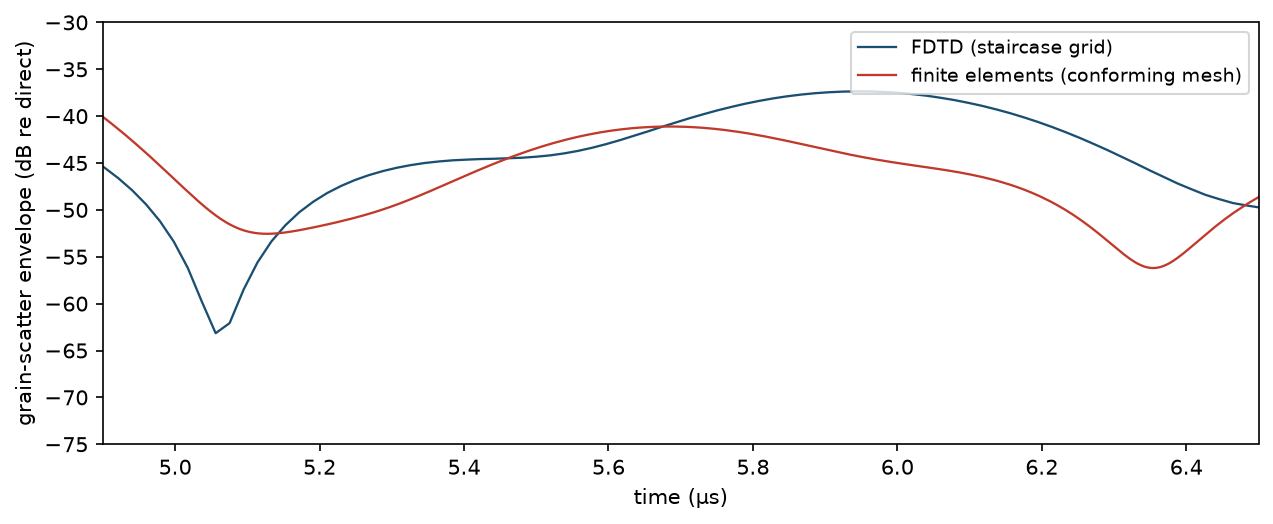
\includegraphics[width=0.95\textwidth]{figures/fe-arbiter.png}
  \caption{The passing arbiter round, reproduced from the archived
    traces: grain-scatter envelopes (specimen minus uniform control,
    each referenced to its own direct arrival) for the FDTD solver
    and the independent finite-element solver over the analysis
    window.}
  \label{fig:arbiter}
\end{figure}
